% Copyright 2026 Sreeram Anil
% SPDX-License-Identifier: CC-BY-4.0
\chapter{Joint state and parameter estimation with a sigma-point filter (Joint SPKF)}
\label{ch:jointukf}

\section*{At a glance}
\begin{tabular}{@{}l>{\raggedright\arraybackslash}p{0.76\textwidth}@{}}
Family & Joint/dual state--parameter estimation (SOH) \\
Header & \texttt{include/estkit/parameter/joint\_ukf.hpp} \\
Registered name & \texttt{JointUKF} \\
State dimension & $n_a = n_x + n_p = 6$; $2n_a+1=13$ sigma points \\
Cost per step & $\mathcal{O}(n_a^3)$ for the Cholesky, $13$ model evaluations; \SI{4.8}{\micro\second}/step measured \\
Primary references & \cite{plett2006spkf2,plett2006spkf1,wan2000ukf,julier2004unscented,ljung1979ekf} \\
\end{tabular}

\section{Motivation and aerospace/BMS relevance}
The joint EKF of Chapter~\ref{ch:jointekf} inherits one structural weakness from its linearisation:
the augmented dynamics are \emph{bilinear} in $(\vx,\vtheta)$ --- the Coulomb-counting term is
$i/Q$, the ohmic term is $R_0 i$ --- and a first-order Taylor expansion of a product is exactly the
term it cannot represent.  Plett introduced sigma-point Kalman filtering to battery management for
precisely this reason~\cite{plett2006spkf1}, and the second part of that work~\cite{plett2006spkf2}
applies it to simultaneous state and parameter estimation.

The sigma-point (unscented) transform replaces the Jacobian by a deterministic sample of $2n_a+1$
points that is propagated through the \emph{exact} nonlinear map.  The resulting mean and
covariance are correct to second order in the Taylor expansion for any nonlinearity, and, crucially
for the joint problem, the state/parameter cross-covariance is obtained without ever differentiating
with respect to $\vtheta$: each sigma point simply evaluates $f$ and $h$ with \emph{its own}
parameter vector.  For an avionics implementation this also removes the numerical-differentiation
step, which is the part of the joint EKF that is hardest to certify (the step size $\delta_j$ is a
magic number and the derivative is only as good as the floating-point cancellation allows).

The costs are a factor $\approx 2n_a$ more model evaluations per step and the need for a Cholesky
factorisation of an augmented covariance whose entries span ten orders of magnitude --- the SOC
variance is $\sim10^{-8}$ while the capacity variance is $\sim10^{-1}$.  Both are manageable, and
the method is the one Plett recommends when the parameters are strongly coupled to the state.

\section{Problem statement and assumptions}
The model class, the augmentation and the assumptions are identical to
Chapter~\ref{ch:jointekf}: the plant is \eqref{eq:je-f}--\eqref{eq:je-h}, the parameters follow the
random walk of Assumption~\ref{as:je-rw}, and the augmented state is
$\bm{\xi}=[\vx^\T,\vtheta^\T]^\T\in\real^{n_a}$ with $n_a=n_x+n_p$.  What changes is only how the
first two moments of $\bm{\xi}$ are propagated: by the scaled unscented transform instead of by a
Jacobian.  The additional assumption is the one that underlies every sigma-point filter.

\begin{assumption}[Moment adequacy]\label{as:ju-moments}
The posterior of $\bm{\xi}_k$ given $\vy_{1:k}$ is adequately described by its first two moments,
and $f_a$, $h_a$ are twice differentiable so that the unscented transform is exact to second order.
\end{assumption}

\section{Derivation}

\subsection{The scaled unscented transform}
Let $\hat{\bm{\xi}}\in\real^{n_a}$ and $\bm{\Pi}\in\real^{n_a\times n_a}$, $\bm{\Pi}\succ0$.  With
the scaling parameters $\alpha\in(0,1]$, $\kappa\ge0$, $\beta\ge0$ and
\begin{equation}
\lambda=\alpha^2(n_a+\kappa)-n_a, \qquad c=n_a+\lambda,
\label{eq:ju-lambda}
\end{equation}
the sigma set and weights are
\begin{align}
\mathcal{X}^{(0)}&=\hat{\bm{\xi}}, &
\mathcal{X}^{(j)}&=\hat{\bm{\xi}}+\left(\sqrt{c\,\bm{\Pi}}\right)_{:,j}, &
\mathcal{X}^{(j+n_a)}&=\hat{\bm{\xi}}-\left(\sqrt{c\,\bm{\Pi}}\right)_{:,j}, \quad j=1..n_a,
\label{eq:ju-sigma}\\
w^{(0)}_m&=\frac{\lambda}{c}, &
w^{(0)}_c&=\frac{\lambda}{c}+1-\alpha^2+\beta, &
w^{(j)}_m&=w^{(j)}_c=\frac{1}{2c},
\label{eq:ju-weights}
\end{align}
where $\sqrt{\cdot}$ denotes a lower-triangular Cholesky factor.  The set matches the mean and
covariance of $\bm{\xi}$ exactly and, for a symmetric distribution, also the third moment; $\beta=2$
is optimal for a Gaussian~\cite{wan2000ukf}.

\subsection{Time update}
Each sigma point is a complete hypothesis ``the state is $\vx^{(j)}$ \emph{and} the parameters are
$\vtheta^{(j)}$''.  Propagating it means evaluating the cell model with those parameters:
\begin{equation}
\mathcal{X}^{(j)}_{k|k-1}
=f_a\!\left(\mathcal{X}^{(j)}_{k-1},\vu_{k-1}\right)
=\begin{bmatrix} f\!\left(\vx^{(j)}_{k-1},\vu_{k-1};\vtheta^{(j)}_{k-1}\right)\\[1mm] \vtheta^{(j)}_{k-1}\end{bmatrix},
\label{eq:ju-prop}
\end{equation}
\begin{equation}
\hat{\bm{\xi}}^-_k=\sum_{j=0}^{2n_a} w^{(j)}_m \mathcal{X}^{(j)}_{k|k-1},
\qquad
\bm{\Pi}^-_k=\sum_{j=0}^{2n_a} w^{(j)}_c\left(\mathcal{X}^{(j)}_{k|k-1}-\hat{\bm{\xi}}^-_k\right)\left(\cdot\right)^\T+\mQ_a .
\label{eq:ju-tu}
\end{equation}
The lower block of \eqref{eq:ju-prop} is the identity, so the parameter mean is unchanged and its
covariance grows by $\bm{\Sigma}_r$ --- exactly as in the joint EKF.  The difference is in the
\emph{cross}-block: because $\vtheta^{(j)}$ varies across the sigma set, the propagated state
points spread by an amount that reflects the true nonlinear dependence of $f$ on $\vtheta$, so
$\mP^-_{x\theta}$ is captured without the derivative \eqref{eq:je-fd}.

\subsection{Measurement update}
With $\mathcal{Y}^{(j)}_k=h\!\left(\vx^{(j)}_{k|k-1},\vu_k;\vtheta^{(j)}_{k|k-1}\right)$,
\begin{align}
\hat{\vy}^-_k&=\sum_j w^{(j)}_m \mathcal{Y}^{(j)}_k, &
\mP_{yy}&=\sum_j w^{(j)}_c\left(\mathcal{Y}^{(j)}_k-\hat{\vy}^-_k\right)\left(\cdot\right)^\T+\mR,\\
\mP_{\xi y}&=\sum_j w^{(j)}_c\left(\mathcal{X}^{(j)}_{k|k-1}-\hat{\bm{\xi}}^-_k\right)\left(\mathcal{Y}^{(j)}_k-\hat{\vy}^-_k\right)^\T, &
\mK_k&=\mP_{\xi y}\mP_{yy}\inv ,
\label{eq:ju-mu}
\end{align}
\begin{equation}
\hat{\bm{\xi}}^+_k=\hat{\bm{\xi}}^-_k+\mK_k\left(\vy_k-\hat{\vy}^-_k\right),
\qquad
\bm{\Pi}^+_k=\bm{\Pi}^-_k-\mK_k\mP_{yy}\mK_k^\T .
\label{eq:ju-mu2}
\end{equation}
The lower $n_p$ rows of $\mP_{\xi y}$ are precisely the empirical covariance between the parameter
hypotheses and the outputs they predict --- the sigma-point replacement for the
$\partial\hat{y}/\partial\vtheta$ of the extended formulation.  For the ECM the $R_0$ rows are
populated immediately (each sigma point predicts a different ohmic drop), whereas the $Q$ rows
accumulate slowly, for the reason given in \eqref{eq:je-dfdQ}: a different capacity changes the
predicted voltage only after it has changed the SOC.

\begin{remark}[Relation to the joint EKF]
If $f_a$ and $h_a$ were affine, \eqref{eq:ju-tu}--\eqref{eq:ju-mu2} would reduce exactly to the
Kalman recursion and hence to Chapter~\ref{ch:jointekf}.  The observable difference in the results
of Section~\ref{sec:ju-results} is therefore entirely attributable to the bilinear terms $i/Q$ and
$R_0 i$.
\end{remark}

\section{Algorithm}
\begin{algorithm}[H]
\caption{Joint SPKF --- one sampling period}
\begin{algorithmic}[1]
\Require $\hat{\bm{\xi}}^+_{k-1}$, $\bm{\Pi}^+_{k-1}$, $\vu_{k-1}$, $\vy_k$, $\vu_k$
\State \textbf{Time update:} build $\{\mathcal{X}^{(j)}\}$ from $(\hat{\bm{\xi}}^+_{k-1},\bm{\Pi}^+_{k-1})$ by \eqref{eq:ju-sigma}
\State $\mathcal{X}^{(j)}_{k|k-1}\gets f_a(\mathcal{X}^{(j)},\vu_{k-1})$ for all $j$ \Comment{each with its own $\vtheta^{(j)}$}
\State $\hat{\bm{\xi}}^-_k,\ \bm{\Pi}^-_k \gets$ \eqref{eq:ju-tu}; symmetrise
\State \textbf{Measurement update:} rebuild $\{\mathcal{X}^{(j)}\}$ from $(\hat{\bm{\xi}}^-_k,\bm{\Pi}^-_k)$
\State $\mathcal{Y}^{(j)}_k\gets h_a(\mathcal{X}^{(j)},\vu_k)$; form $\hat{\vy}^-_k,\mP_{yy},\mP_{\xi y}$ by \eqref{eq:ju-mu}
\State $\mK_k\gets\mP_{\xi y}\mP_{yy}\inv$; apply \eqref{eq:ju-mu2}; symmetrise
\State project: $\xplus_k\gets\mathrm{constrain}(\xplus_k)$, $\hat{\vtheta}^+_k\gets$ box
\Ensure $\hat{\bm{\xi}}^+_k,\ \bm{\Pi}^+_k$
\end{algorithmic}
\end{algorithm}

\section{Application to the battery model}
The class is a thin wrapper around \texttt{Ukf<AugmentedModel<EcmModel>{}>} with exactly the same
\texttt{init()} convention and the same prior and random-walk settings as the joint EKF
(Section~\ref{sec:je-app}): $p_{0,Q}=(0.10\,Q_\text{nom})^2$, $q_Q=(\SI{5e-5}{\ampere\hour})^2$ per
step, $p_{0,R_0}=(0.30\,R_{0,\text{nom}})^2$, $q_{R_0}=(\SI{2e-6}{\ohm})^2$ per step, with the same
boxes.  Using identical tuning is deliberate: the two chapters then differ only in how the moments
are propagated, which makes the comparison in Section~\ref{sec:ju-results} meaningful.

The unscented parameters are $\alpha=0.1$, $\beta=2$, $\kappa=0$, inherited from the state-only UKF
so that the two are comparable.  With $n_a=6$ this gives $\lambda=\alpha^2 n_a-n_a=-5.94$ and
$c=0.06$, i.e.\ sigma points at $\pm0.245\sigma$ and a large negative centre weight.  This is the
``small-$\alpha$'' regime in which the unscented transform behaves like a central-difference
linearisation; it is the standard choice when the state is well conditioned and the nonlinearity is
mild over one sampling period, which is the case here ($\dt=\SI{0.1}{\second}$).  The centre point
contributes nothing to $\bm{\Pi}^-$ in the time update (its deviation is zero by construction), so
the negative weight is harmless.

The Cholesky factorisation in \eqref{eq:ju-sigma} operates on a matrix whose diagonal spans
$\mP_{\soc\soc}\approx3\times10^{-8}$ to $\mP_{QQ}=0.25$, a condition number of order $10^{7}$.
The library's \texttt{cholesky\_safe} adds a relative jitter of $10^{-12}(1+\|\bm{\Pi}\|_\infty)$
and retries on failure, which is sufficient in double precision; the single-precision build is also
stable here, but a square-root sigma-point filter (SR-UKF) would be the correct choice for a
production flight build.

\section{Implementation notes}
Memory is \SI{5496}{\byte} for the registered estimator: the $6\times6$ covariance, thirteen
$6$-vectors of sigma points and two copies of the cell parameters.  There is no heap allocation.
Per step the filter performs two Cholesky factorisations of a $6\times6$ matrix and $2\times13$
model evaluations; because \texttt{AugmentedModel::with()} copies the whole \texttt{EcmModel}
(including its \SI{3.9}{\kilo\byte} OCV table) for every sigma point, the measured cost is
\SI{4.8}{\micro\second}/step --- about $2.6\times$ the joint EKF and $10\times$ the plain
EKF --- and is dominated by \texttt{memcpy}, not by arithmetic.  Sharing the OCV table by reference
would remove most of it; on a Cortex-M7 with the table in flash the true cost is the $13$ model
evaluations, i.e.\ roughly the cost of thirteen EKF propagations.

The known weaknesses are those of any joint estimator: an unmodelled residual is spent on
$\vtheta$, and the filter has no mechanism to distinguish ``the model is wrong'' from ``the
parameters are wrong''.  The sigma-point formulation does not change that; it only removes the
linearisation error.

\section{Benchmark results}
\label{sec:ju-results}
% Copyright 2026 Sreeram Anil
% SPDX-License-Identifier: CC-BY-4.0
\begin{table}[H]\centering\footnotesize\setlength{\tabcolsep}{4pt}
\caption{JointUKF: cell-level benchmark on the eVTOL mission (mean over seeds; RMSE and max error in \% SOC; $t_\mathrm{conv}$: first time the error stays below 2\,\% for 60\,s, -- = never; EKF reference: steady-state RMSE of the plain EKF on the same data).}\label{tab:cell_JointUKF}
\begin{tabular}{llrrrrrcrr}\toprule
plant & scenario & RMSE & RMSE$_\mathrm{ss}$ & max & $t_\mathrm{conv}$ [s] & RMSE$_v$ [mV] & div. & EKF ref. & ns/step \\ \midrule
ECM & nominal & 0.15 & 0.11 & 4.02 & 0 & 1.09 & no & 0.05 & 3103 \\
ECM & init\_error & 0.76 & 0.05 & 3.80 & 128 & 2.06 & no & 0.05 & 3123 \\
ECM & current\_bias & 0.56 & 0.58 & 3.83 & 0 & 1.08 & no & 0.61 & 3099 \\
ECM & noise\_step & 0.47 & 0.55 & 4.02 & 0 & 3.01 & no & 0.12 & 3096 \\
ECM & outliers & 1.08 & 0.37 & 5.50 & 238 & 2.28 & no & 0.21 & 3096 \\
ECM & cold & 0.30 & 0.16 & 3.97 & 1 & 2.09 & no & 0.16 & 3096 \\
ECM & hot & 0.16 & 0.08 & 4.04 & 0 & 0.91 & no & 0.03 & 3090 \\
ECM & aged\_cell & 0.18 & 0.06 & 4.37 & 0 & 1.30 & no & 1.52 & 3098 \\
ECM & param\_mismatch & 1.66 & 0.49 & 7.08 & 0 & 1.26 & no & 1.36 & 3090 \\
ECM & sensor\_dropout & 1.88 & 1.86 & 8.57 & 0 & 1.93 & no & 0.46 & 3109 \\
ECM & preisach & 1.67 & 0.94 & 6.58 & 219 & 1.20 & no & 0.20 & 3102 \\
ECM & combined & 2.15 & 1.51 & 7.93 & 225 & 2.36 & no & 12.44 & 3100 \\
\midrule
SPM & nominal & 2.49 & 1.40 & 5.95 & 0 & 1.13 & no & 3.73 & 3012 \\
SPM & init\_error & 2.38 & 0.82 & 6.22 & 557 & 2.01 & no & 3.81 & 3010 \\
SPM & current\_bias & 2.51 & 1.51 & 5.87 & 0 & 1.11 & no & 5.69 & 3007 \\
SPM & noise\_step & 3.76 & 4.28 & 8.17 & 0 & 3.20 & no & 3.30 & 3022 \\
SPM & outliers & 5.06 & 6.29 & 8.88 & 95 & 2.50 & no & 1.99 & 3017 \\
SPM & cold & 4.02 & 2.49 & 8.36 & 1480 & 2.40 & no & 7.35 & 2973 \\
SPM & hot & 1.18 & 0.48 & 4.43 & 0 & 0.93 & no & 2.16 & 3012 \\
SPM & param\_mismatch & 2.17 & 0.92 & 5.58 & 194 & 1.14 & no & 3.13 & 3012 \\
SPM & sensor\_dropout & 3.66 & 2.20 & 8.76 & 0 & 2.00 & no & 5.31 & 2981 \\
\bottomrule\end{tabular}\end{table}
\begin{table}[H]\centering\small\caption{JointUKF: additional outputs (capacity error at the end of the mission in Ah, averaged over the last 10\,\% of the run; interval-bound violation rate).}\label{tab:cellx_JointUKF}
\begin{tabular}{llrr}\toprule plant & scenario & $\hat Q - Q$ [Ah] & bound violation [\%] \\ \midrule
ECM & nominal & +0.031 & -- \\
ECM & init\_error & +0.060 & -- \\
ECM & current\_bias & +0.311 & -- \\
ECM & noise\_step & +0.066 & -- \\
ECM & outliers & -0.054 & -- \\
ECM & cold & +0.036 & -- \\
ECM & hot & +0.041 & -- \\
ECM & aged\_cell & +0.039 & -- \\
ECM & param\_mismatch & -0.328 & -- \\
ECM & sensor\_dropout & +0.497 & -- \\
ECM & preisach & +0.229 & -- \\
ECM & combined & +0.240 & -- \\
SPM & nominal & +0.219 & -- \\
SPM & init\_error & +0.534 & -- \\
SPM & current\_bias & +0.431 & -- \\
SPM & noise\_step & +0.732 & -- \\
SPM & outliers & +0.500 & -- \\
SPM & cold & +0.075 & -- \\
SPM & hot & +0.264 & -- \\
SPM & param\_mismatch & +0.487 & -- \\
SPM & sensor\_dropout & +0.492 & -- \\
\bottomrule\end{tabular}\end{table}

\begin{figure}[H]\centering
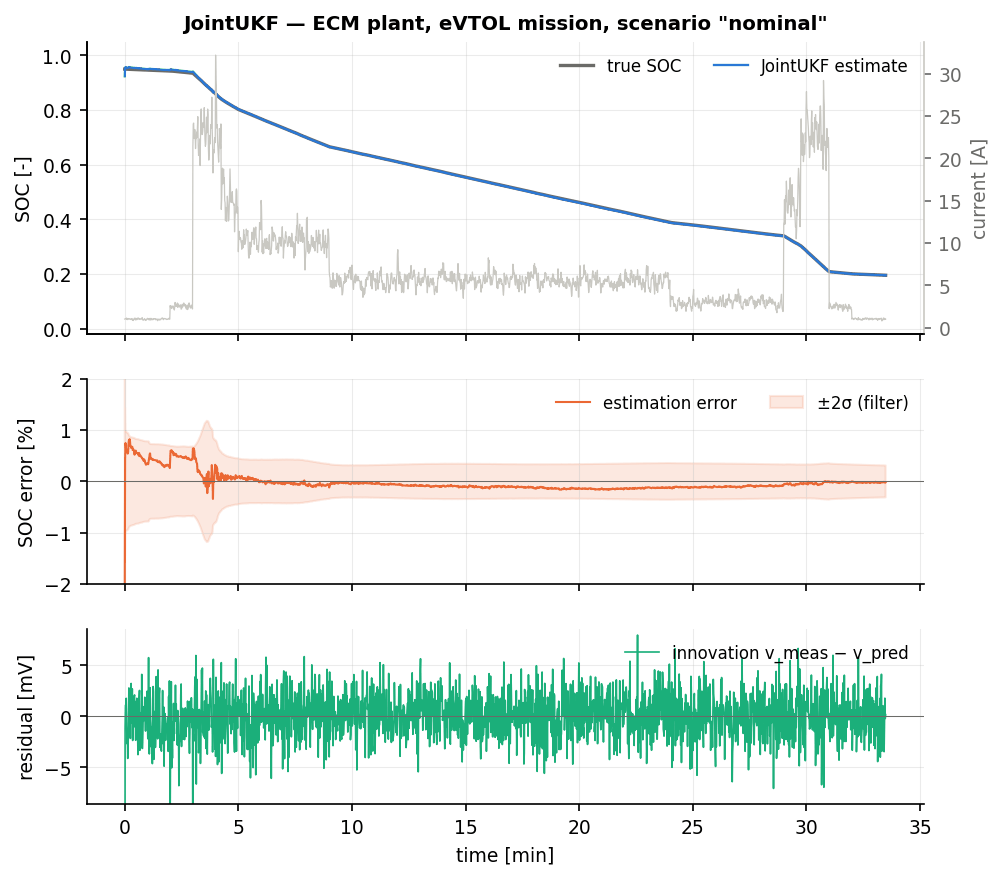
\includegraphics[width=\textwidth]{figures/cell_JointUKF_nominal.png}
\caption{JointUKF on the nominal eVTOL mission: true and estimated SOC (top), estimation error with the $\pm 2\sigma$ band (middle), voltage residual (bottom).}
\end{figure}
\begin{figure}[H]\centering
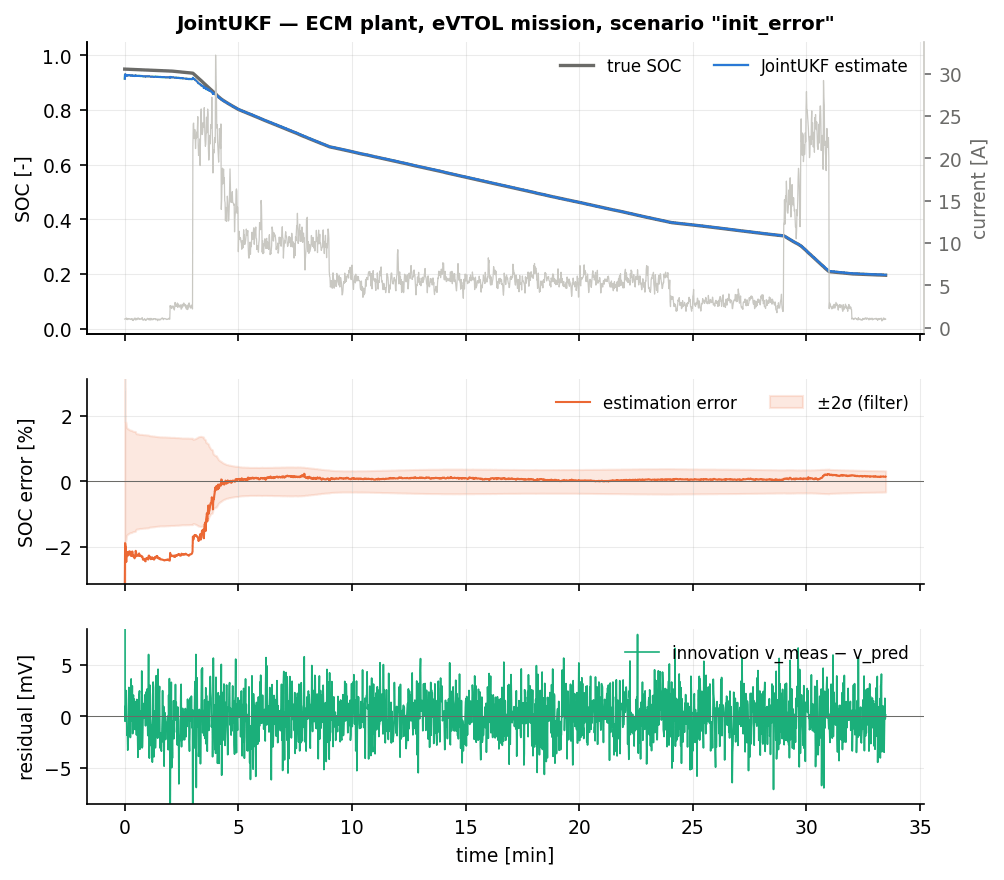
\includegraphics[width=\textwidth]{figures/cell_JointUKF_init_error.png}
\caption{JointUKF with a \SI{35}{\percent} initial SOC error.}
\end{figure}

All figures below are means over three seeds on the eVTOL profile.  On \texttt{nominal} the joint
SPKF reaches $\text{RMSE}=0.0015$ and $\text{RMSE}_\text{ss}=0.0011$ with convergence at
$t=\SI{0.5}{\second}$, against $0.0020/0.0004$ for the plain UKF and $0.0015/0.0005$ for the plain
EKF in the same run.  On \texttt{init\_error} (a \SI{35}{\percent} initial SOC error) the
run-average RMSE is $0.0076$ and the steady-state value $0.0005$, but the convergence time is
\SI{128}{\second} --- by far the slowest of the six SOH methods.  The reason is visible in the tuning: with $\alpha=0.1$ and $n_a=6$ the sigma points sit at
$0.245\sigma$, so the effective spread of the augmented state is small, and the filter needs many
samples before the parameter block and the large initial SOC error stop competing to explain the
same residual.  The acceptance criterion (convergence with no divergence) is met, but a
practitioner who cares about cold-start time should either raise $\alpha$ or hold the parameter
block frozen for the first minute.

On \texttt{aged\_cell} the method matches the joint EKF: $\text{RMSE}_\text{ss}=0.0006$
against the plain EKF's $0.0152$ and the plain UKF's $0.0136$, with
$\texttt{capacity\_err\_end}=\SI{+0.039}{\ampere\hour}$, i.e.\ about \SI{4.27}{\ampere\hour}
recovered from a true \SI{4.23}{\ampere\hour}.  The three reference capacity figures are
\begin{center}
\begin{tabular}{@{}lrr@{}}
\toprule
Scenario & $Q_\text{true}$ (\si{\ampere\hour}) & \texttt{capacity\_err\_end} (\si{\ampere\hour})\\
\midrule
\texttt{nominal}      & 5.00 & $+0.031$\\
\texttt{aged\_cell}   & 4.25 & $+0.039$\\
\texttt{current\_bias}& 5.00 & $+0.311$\\
\bottomrule
\end{tabular}
\end{center}
The \texttt{current\_bias} value is within \SI{11}{\milli\ampere\hour} of the joint EKF's, which is
the expected outcome: the bias is a property of the \emph{problem} (capacity and current-sensor gain
enter only as the product $\alpha i/Q$, cf.\ \cite{zhao2017observability,lin2018sensorbias}), not of
the estimator, so two correctly implemented estimators must agree on it.  That they do is a useful
cross-check on both implementations.

Where the sigma-point version earns its extra cost is the scenarios in which the residual is
\emph{not} a clean parameter error.  On \texttt{param\_mismatch} the steady-state SOC error is by far the best of the twelve estimators
compared ($0.0049$ against the joint EKF's $0.0120$ and the plain EKF's $0.0136$) --- but the
capacity is pushed \SI{0.328}{\ampere\hour} \emph{low}, in the opposite direction to the joint
EKF's \SI{+0.102}{\ampere\hour}.  The two estimators are both absorbing an unmodelled $R_1$ and
$\tau_2$ error into $(Q,R_0)$ and they simply land in different local minima of the same
prediction-error criterion; this is exactly the non-uniqueness Ljung warns about~\cite{ljung1979ekf}
and it is a reminder that a capacity estimate is only as trustworthy as the rest of the model.
\texttt{sensor\_dropout} is the worst column for both joint filters
($\text{RMSE}_\text{ss}=0.0186$, $\texttt{capacity\_err\_end}=\SI{+0.497}{\ampere\hour}$): a
\SI{15}{\second} stuck voltage during the take-off hover is integrated straight into the parameter
block.  On \texttt{combined} the joint SPKF is clearly the better of the two ($0.0215/0.0151$
against $0.0383/0.0258$), consistent with the plain UKF also handling that scenario much better
than the plain EKF ($0.0123$ against $0.1602$).

\paragraph{The electrochemical plant.}  On the SPM plant, where the estimator's ECM carries a
structured few-millivolt model error, the joint SPKF is the best of the two joint filters and the
second best estimator overall: $\text{RMSE}_\text{ss}=0.0140$ on \texttt{nominal} against the plain
UKF's $0.0396$, the plain EKF's $0.0373$ and the joint EKF's $0.0211$, and $0.0082$ on
\texttt{init\_error}, the best figure any estimator achieves on that plant for that scenario.  Its
one weak SPM column is \texttt{outliers} ($0.0629$ against the plain UKF's $0.0176$), where the
combination of a heavy-tailed measurement and an unmodelled plant is more than the augmented
covariance can absorb.

\paragraph{Multi-flight capacity tracking.}  Over the 120-flight accelerated ageing study
(\texttt{bench\_soh --flights 120 --accel 3}) it tracks the fading capacity with an RMSE of
\SI{29}{\milli\ampere\hour} and a final error of \SI{+22}{\milli\ampere\hour}, with the lowest mean
per-flight SOC RMSE of the family ($0.0010$) --- but at \SI{5.3}{\micro\second}/step it is also by
far the most expensive of the five.

Cost: \SI{4.8}{\micro\second}/step and \SI{5496}{\byte}.

\section{Summary}
The joint SPKF gives the same capacity accuracy as the joint EKF --- \SI{0.039}{\ampere\hour} on
the aged cell, \SI{29}{\milli\ampere\hour} over a 120-flight ageing study --- while removing the
parameter Jacobian, and it is markedly better on the \texttt{combined} scenario, under parameter
mismatch, and on the electrochemical plant, where it is the second most accurate estimator in the
whole benchmark.  It costs about $2.6\times$ the joint EKF.  Prefer it when the parameter/state coupling is strong (large
C-rates, large SOC swings), when the analytic or numerical Jacobians of the augmented model are
awkward to certify, or when the data are noisy.  Avoid it if cold-start convergence time matters:
with the inherited $\alpha=0.1$ tuning it needs \SI{128}{\second} to recover a \SI{35}{\percent}
initial SOC error, whereas the extended version is immediate.  Neither joint filter should be
trusted when the current-sensor scale factor is unknown or when sensor faults are possible.
